\documentclass[aspectratio=43]{beamer}

\usetheme{simple}

\usepackage{lmodern}
\usepackage[scale=2]{ccicons}

\usepackage[utf8]{inputenc}


\def\edicion{XXXV}
\def\fecha{Abril 2023}

\title{Te has instalado Linux... ahora, ¿qué?} % título de la presentación
\author{Luis Daniel Casais} % autor de la presentación
\github{rajayonin} % GitHub

\institute{\edicion \ Jornadas Técnicas del GUL}
\date{\fecha}


\titlegraphic{img/logo1.png}


% -----------------------------
% La presentación empieza aquí.
% -----------------------------


\begin{document}

{
    \setbeamertemplate{footline}{}
    \begin{frame}
        \titlepage
    \end{frame}
}
\addtocounter{framenumber}{-1}


\begin{frame}
    \frametitle{Tabla de contenidos}
    \tableofcontents
\end{frame}


\section{Personalización}
% Desktop Enviroments / tiling window managers (i3) / tty
% Emuladores de terminal: kitty (bonito y simple, usa GPU), terminator (GUI friendly), alarcritty (moderno, usa GPU), iterm2 // tmux
% Shells: bash, zsh, fish
% Dotfiles: .bashrc, etc


\begin{frame}
    \frametitle{GUI (Graphical User Interface)}
    Por defecto, Linux cuenta con tres tipos principales de GUI: \textbf{Lockscreen} (pantalla de bloqueo), \textbf{Desktop Enviroment}, y \textbf{TTY/shell}.\newline

    Se puede acceder a cualquiera de ellos con las siguientes combinaciones de teclas:
    \begin{itemize}
        \item \texttt{CTRL + ALT + F1}: Lockscreen
        \item \texttt{CTRL + ALT + F2}: Desktop Environment
        \item \texttt{CTRL + ALT + F3}: TTY3
        \item \texttt{CTRL + ALT + F4}: TTY4\\
        ...\newline
    \end{itemize}
    
    Cualquiera de los tres tipos son personalizables e intercambiables, ya que \textbf{LINUX ES EL AMO Y SEÑOR DE LA PERSONALIZACIÓN}.
\end{frame}

\subsection{Desktop Enviroments}

\begin{frame}
    \frametitle{Desktop Enviroments}
    Es la principal forma de interacción con el ordenador.\\
    Todo lo que puedes ver y tocar (iconos, ventanas, \textit{toolbars}, \textit{wallpapers}, etc.) es parte del Desktop Enviroment.\newline

    Son todos intercambiables y, aunque la forma de hacerlo depende de la \textit{distro} específica, normalmente se pueden cambiar en la \textit{lockscreen}.\\
    Algunas \textit{distros} incluso te permiten elegir cual usar al instalar el SO.\newline

    Hay dos tipos principales, dependiendo de cómo manejan el uso de las ventanas: \textbf{Floating Window Managers} y \textbf{Tiling Window Managers}.
\end{frame}

\begin{frame}
    \frametitle{Floating Window Managers}
    La típica interfaz de un Sistema Operativo moderno, con ventanas "flotantes". Intuitivo y fácil de usar.\newline

    % images
    \begin{columns}[c]
        \begin{column}{0.5\textwidth}
            \begin{figure}
                \centering
                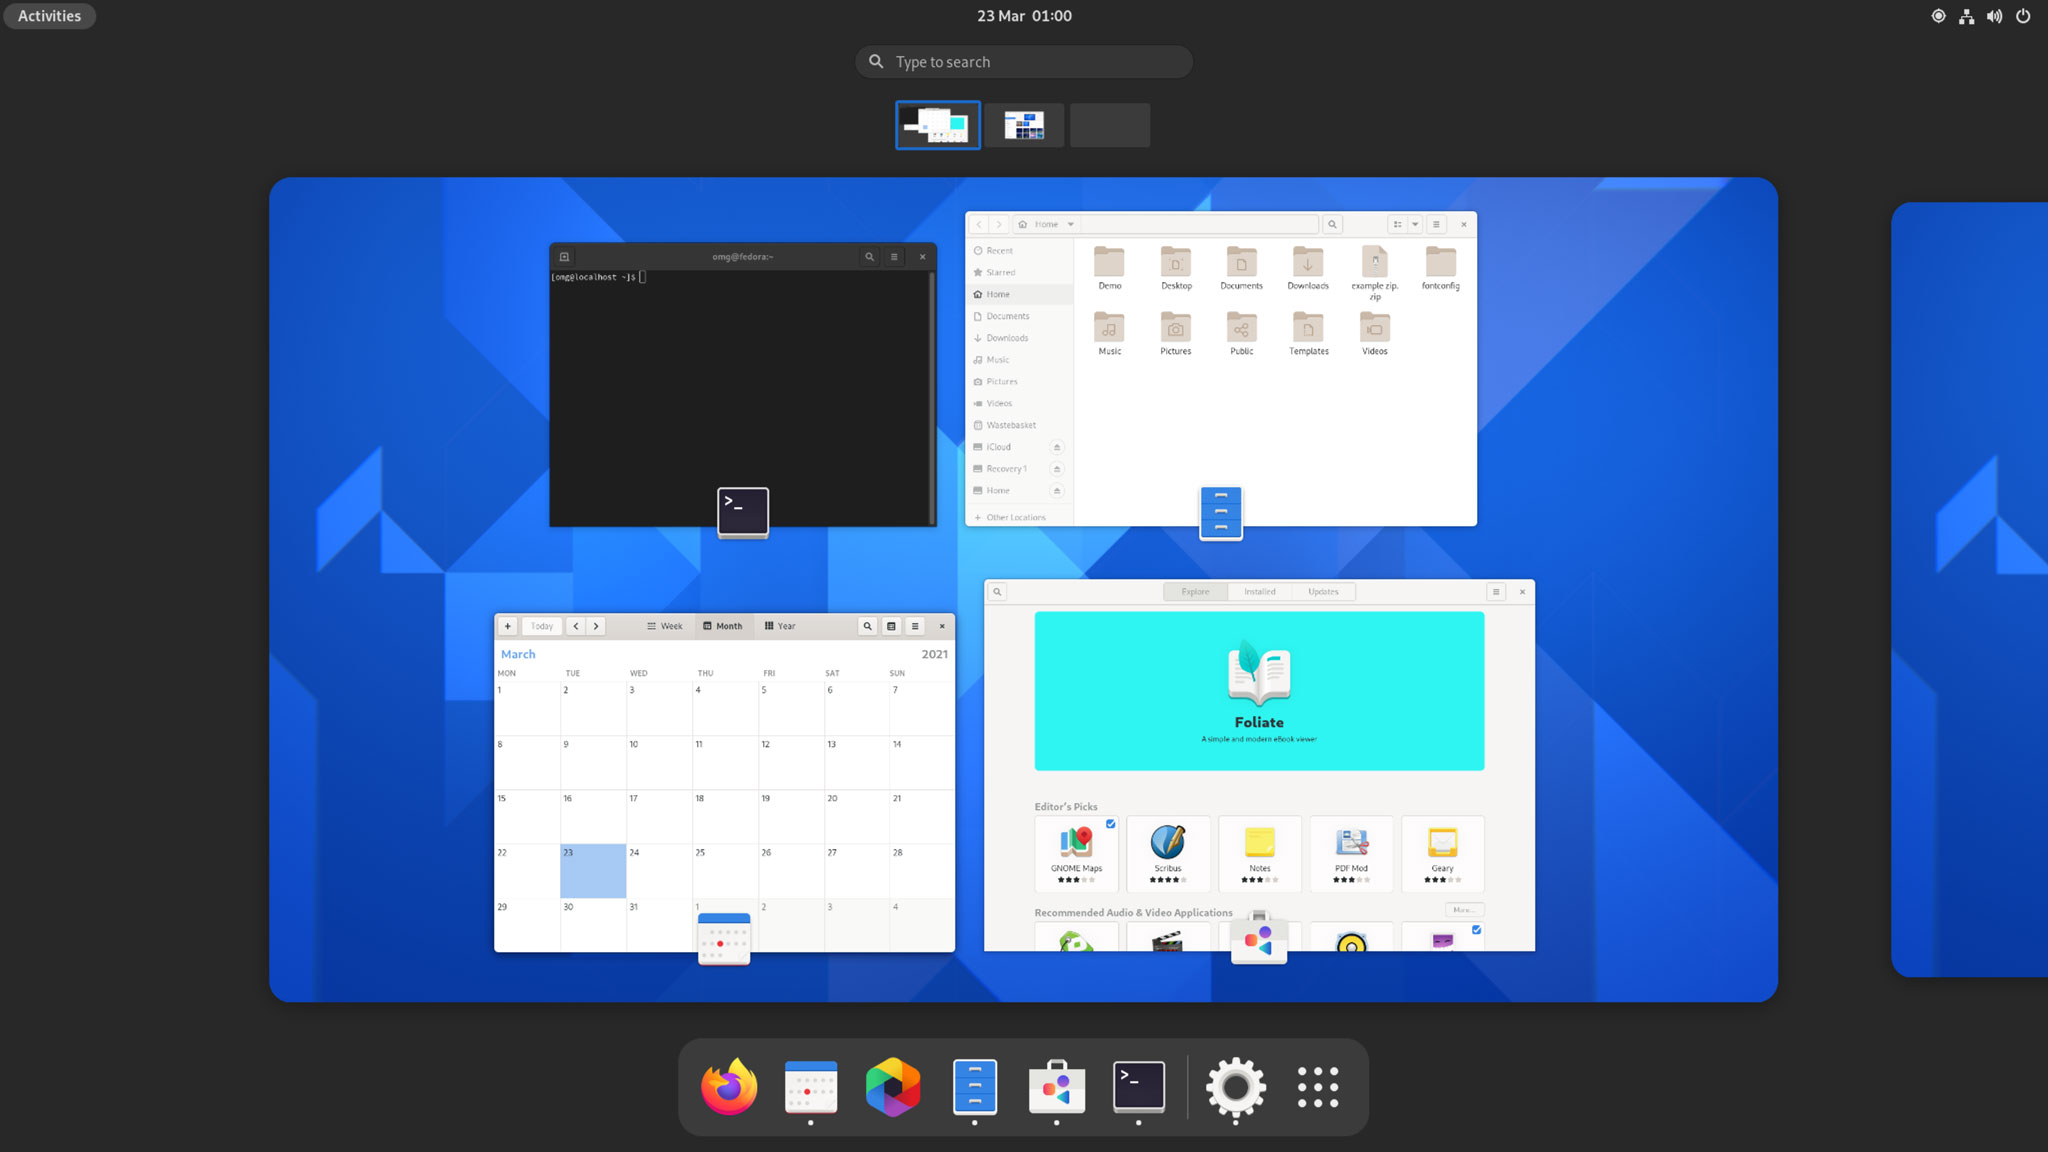
\includegraphics[width=0.9\textwidth]{img/gnome-desktop.jpg}
                \caption{\href{https://forty.gnome.org/}{Gnome 40 Desktop}}
            \end{figure}
        \end{column}
        \begin{column}{0.5\textwidth}
            \begin{figure}
                \centering
                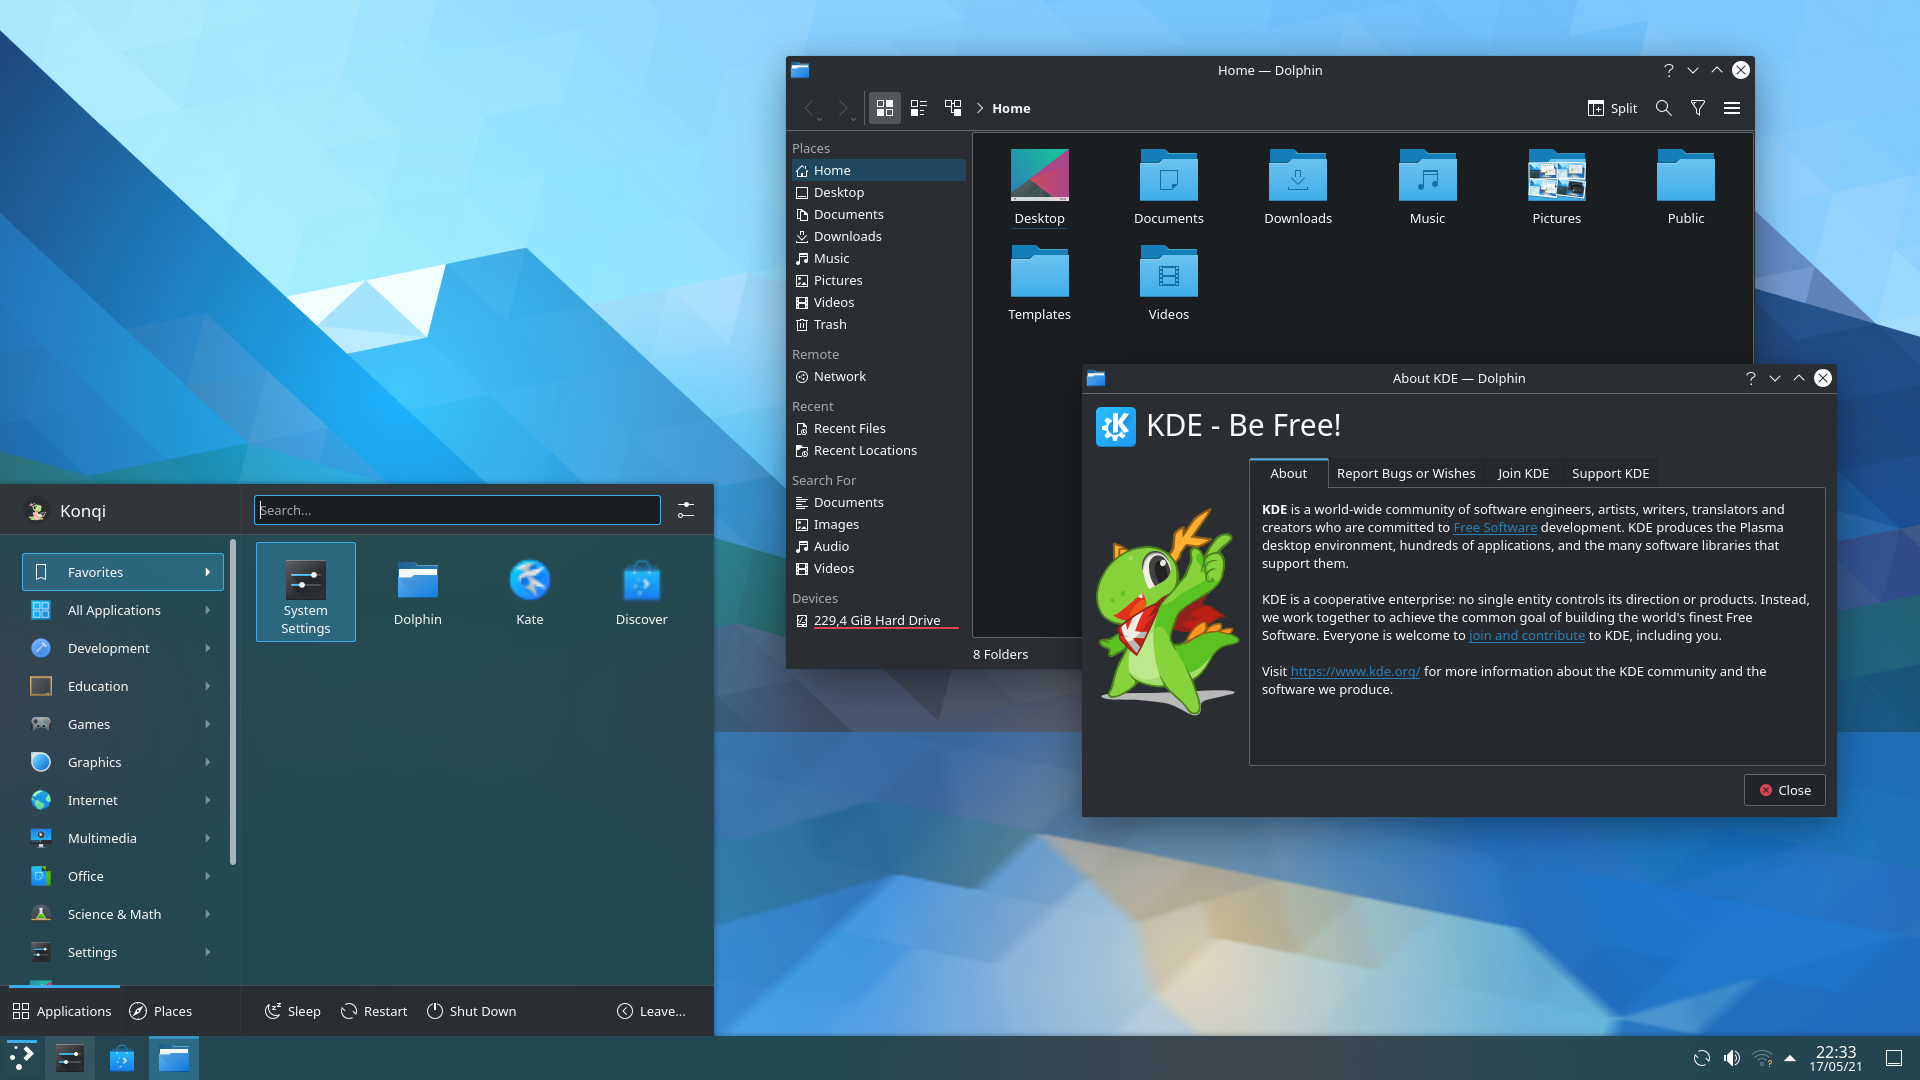
\includegraphics[width=0.9\textwidth]{img/kde_plasma.png}
                \caption{\href{https://kde.org/es/plasma-desktop/}{KDE Plasma Desktop}}
            \end{figure}
        \end{column}
    \end{columns}

\end{frame}

\begin{frame}
    \frametitle{Tiling Window Managers}
    Máximo uso del espacio de la pantalla, 100\% del tiempo (automático). Infinito control y personalización del escritorio.\\
    Todo con \textit{hotkeys} (ratón pa' qué?), pero más difícil de aprender.

    \begin{figure}
        \centering
        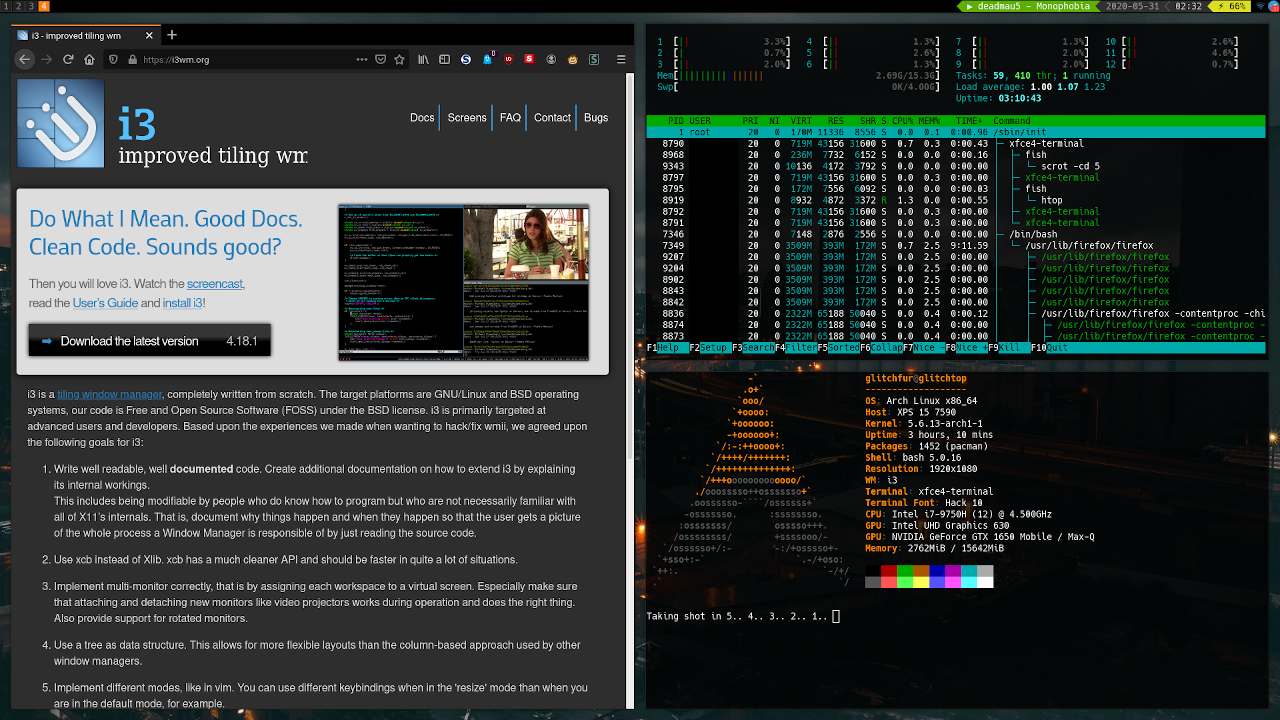
\includegraphics[width=0.6\textwidth]{img/i3_window_manager.png}
        \caption{\href{https://i3wm.org/}{i3 Window Manager}}
    \end{figure}
\end{frame}


\subsection{Emuladores de terminal}
\begin{frame}
    \frametitle{Emuladores de terminal}
    Permiten interactuar con la terminal real, y añaden muchas funcionalidades (copiar y pegar, múltiples terminales...).\newline
    
    % images
    \begin{columns}[c]
        \begin{column}{0.5\textwidth}
            \begin{figure}
                \centering
                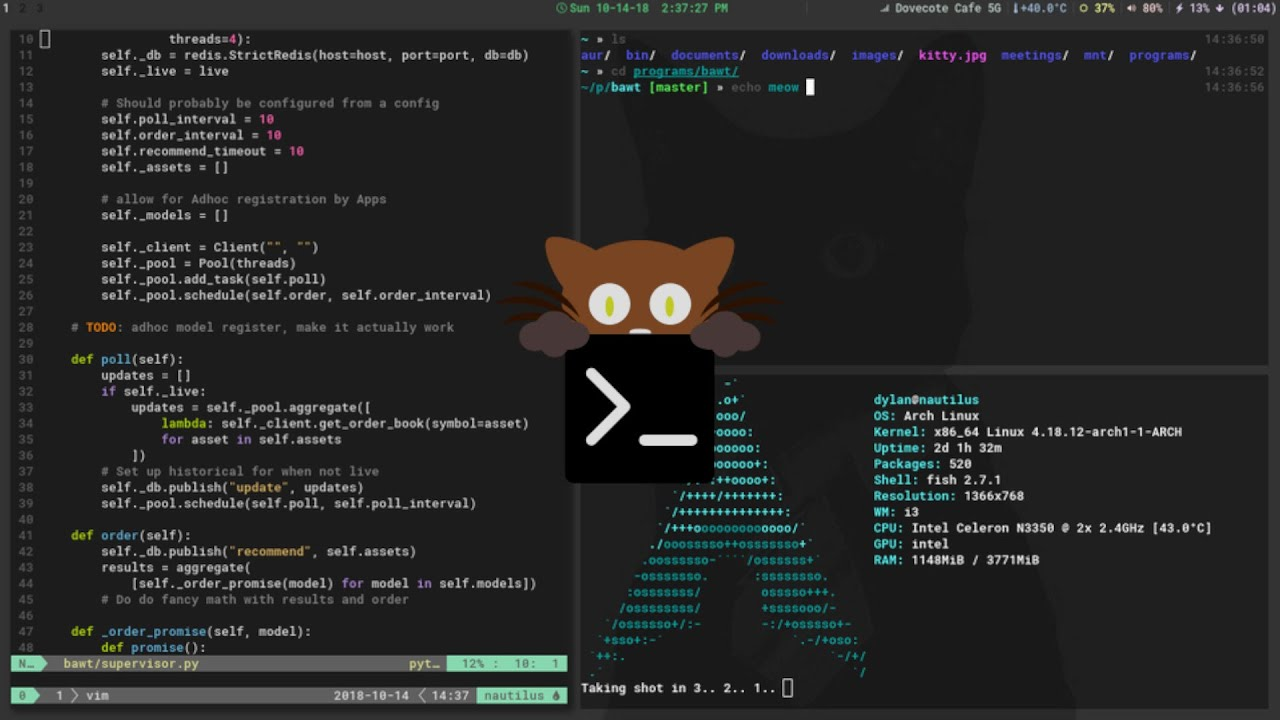
\includegraphics[width=0.9\textwidth]{img/kitty_terminal.jpg}
                \caption{\href{https://sw.kovidgoyal.net/kitty/}{Kitty}}
            \end{figure}
        \end{column}
        \begin{column}{0.5\textwidth}
            \begin{figure}
                \centering
                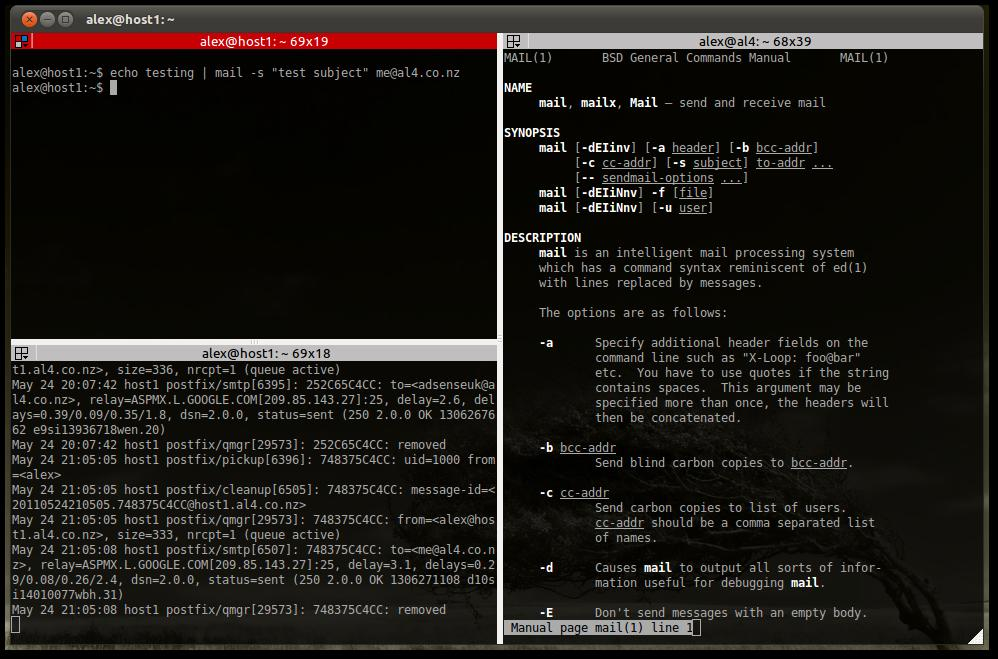
\includegraphics[width=0.9\textwidth]{img/terminator_terminal.jpg}
                \caption{\href{https://gnome-terminator.org/}{Terminator Terminal Emulator}}
            \end{figure}
        \end{column}
    \end{columns}

\end{frame}

\subsection{Shells}

\begin{frame}
    \frametitle{Shells}
    Existen distintos programas de terminal, con distintas funcionalidades (configuración, autocompletado, plugins, etc.).\\
    Son extremadamente fáciles de intercambiar (\href{https://man7.org/linux/man-pages/man1/chsh.1.html}{\texttt{chsh}}), y aún más rápido de arrancar una u otra (son programas: e.g. \href{https://www.man7.org/linux/man-pages/man1/bash.1.html}{\texttt{bash}}). 

    % images
    \begin{columns}[c]
        \begin{column}{0.5\textwidth}
            \begin{figure}
                \centering
                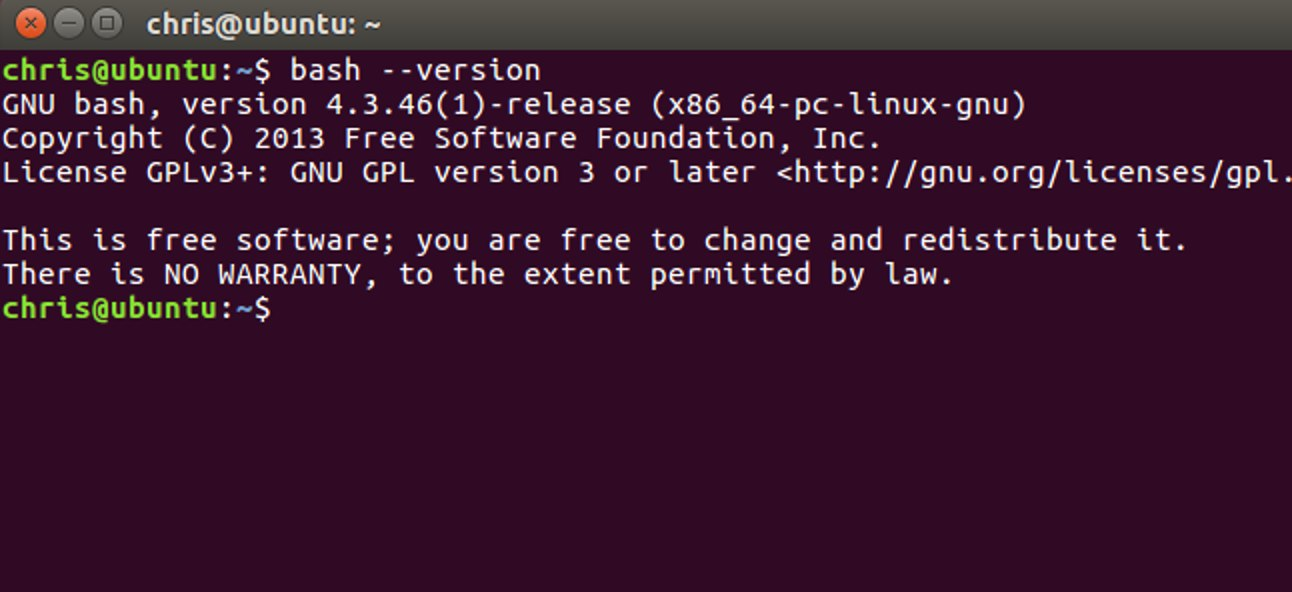
\includegraphics[width=0.9\textwidth]{img/bash_shell.jpg}
                \caption{Bash}
            \end{figure}
        \end{column}
        \begin{column}{0.5\textwidth}
            \begin{figure}
                \centering
                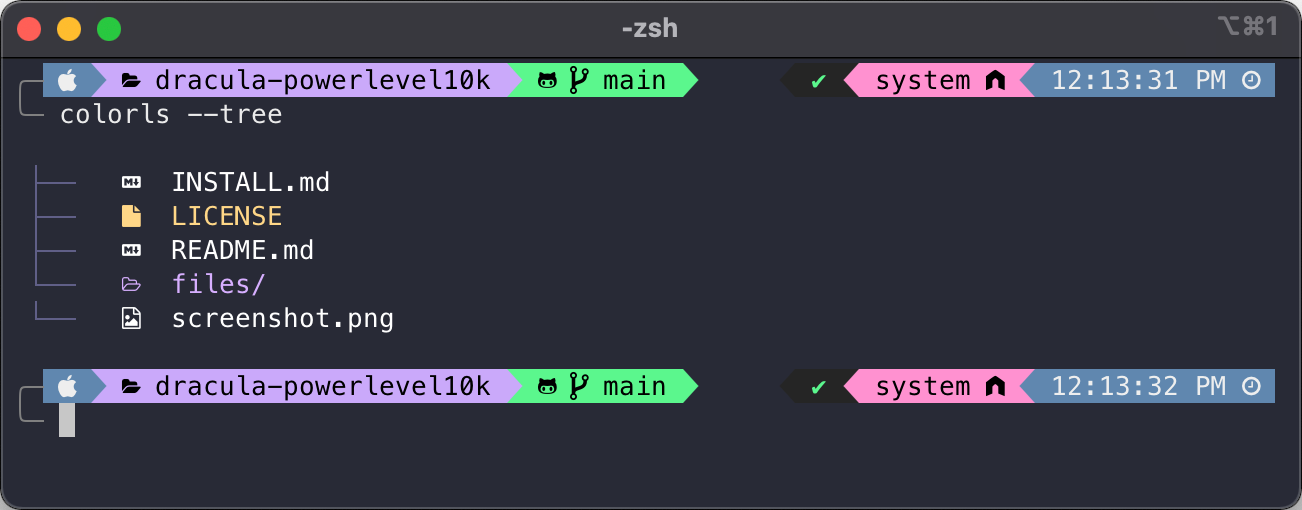
\includegraphics[width=0.9\textwidth]{img/powerlevel10k.png}
                \caption{\href{https://www.zsh.org/}{Z-Shell }\href{https://github.com/romkatv/powerlevel10k}{(with powerlevel10k)}}
            \end{figure}
        \end{column}
    \end{columns}

\end{frame}


\subsection{Dotfiles}

\begin{frame}
    \frametitle{Dotfiles}
    En Linux la mayoría de aplicaciones \textbf{guardan su configuración en archivos de texto plano}, ya sea en \texttt{/etc/} o en \texttt{/home/<user>}, y suelen llamarse "\texttt{.<program>rc}", de ahí su nombre de "\textit{resource files}" o "\textit{dotfiles}".\newline

    Ésto hace que crear, modificar, y compartir configuraciones sea muy sencillo y poderoso (\textit{scripting}, \href{https://github.com/rajayonin/dotfiles}{repositorios}, ...).

    \begin{figure}
        \centering
        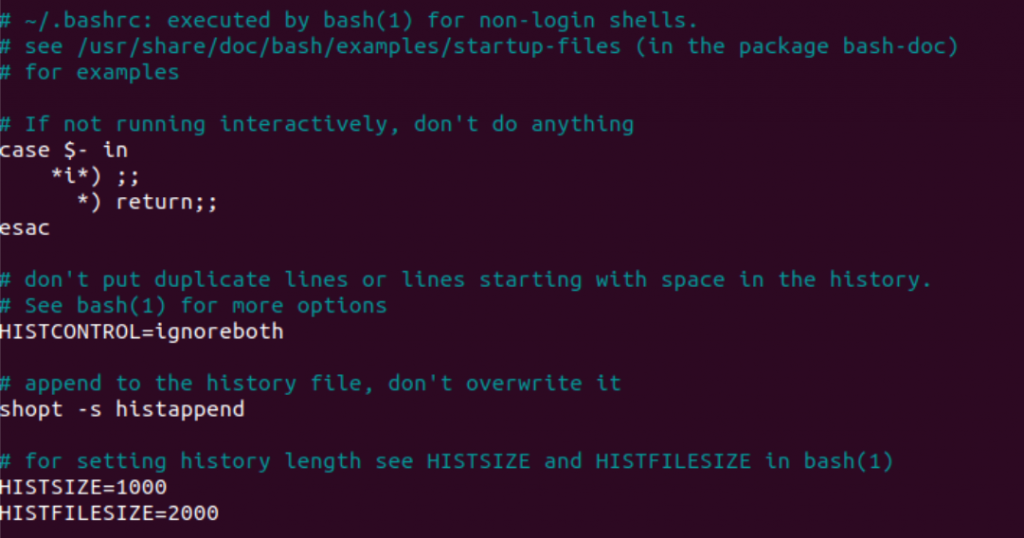
\includegraphics[width=0.4\textwidth]{img/bashrc.png}
        \caption{.bashrc}
    \end{figure}


\end{frame}


\section{La shell}
% Sintaxis: flags, parámetros, y argumentos
% Contraseñas no se muestran en pantalla, Ctrl-L, Ctrl-C, Ctrl-Shift-C, Ctrl-Shift-V
% Funcionalidades de shell: |, >>, >, &&, &, nohup, Ctrl-z, fg
% Shell scripts
% Comandos (https://www.youtube.com/watch?v=s3ii48qYBxA, https://www.youtube.com/watch?v=PeCBpI1hT2Q&t=19s): 
% - Basic: ls, mv, cp, rm, cd, mkdir
% - Coreutils (https://www.maizure.org/projects/decoded-gnu-coreutils/): find/whereis, who, grep, echo, chmod, touch, cat, xxd, history, sudo, df, script
%   - Work w/ files: less, head, tail, sort, comm (diff/cmp), sed/awk, wc, cut, expand/unexpand, tee, jq, yq, xmlint
% - Processes: top (htop) / ps, lscpu,service, kill/kilall
% - Network: ping, traceroute, ipconfig, wget
% - File system: mount, fdisk/gparted, zip/unzip/tar
% - Other: lscpu, neofetch
% - Coña: cowsays, fortune, sl, cmatrix, lolcat, fortune | cowsay -f tux | lolcat (https://www.youtube.com/watch?v=iAdpkqLD4f0)
% Editores de texto en terminal: nano/micro, vim/nvim (lazyvim), emacs
% Reemplazos de comandos: exa, bat
% Configurar terminal: aliases, PS1 (prompt)

\begin{frame}
    \frametitle{}
    
\end{frame}


\section{Más paquetes}
% Más gestores de paquetes: flatpak, snapd (malo), nix, nala (pa debian) 
% LSW ("Linux Subsystem for Windows"): wine, Lutris, heroic games, steam (proton)

\begin{frame}
    \frametitle{}
    
\end{frame}


\section{Configuración y ayuda}
% Ficheros de configuración: /etc/hosts
% Aiuda: man, --help, whatis

\begin{frame}
    \frametitle{}
    
\end{frame}


\section{Acceso remoto}
% ssh, scp


\begin{frame}
    \frametitle{}
    
\end{frame}



\section{Backups}
% rclone: https://www.howtogeek.com/451262/how-to-use-rclone-to-back-up-to-google-drive-on-linux/

\begin{frame}
    \frametitle{}
    
\end{frame}


\section{Ruegos y preguntas}

\begin{frame}
    \frametitle{¿Preguntas, reclamos, improperios?}
    \centering
    
\includegraphics[width=0.9\textwidth]{img/noot.png}
\end{frame}


\begin{frame}
    \frametitle{QR}
    
\end{frame}


\end{document}
